% =====================================================================
%  Relativistic modification of Chapter VIII, §§77–78
%  Stability with transverse pressure gradient — relativistic
% =====================================================================
%
%  Classical reference: Chandrasekhar, Ch. VIII §§77–78,
%    eqs. (8-36)–(8-65) [transverse pressure gradient + rotation]
%  Relativistic framework: BDNK first-order causal dissipation
%  Agent: 35 (subagent for general flow, part 2 — transverse gradient)
% =====================================================================

\section{Relativistic stability of viscous flow between rotating cylinders
  with a transverse pressure gradient}
\label{sec:rel-77}

In the classical theory (\S\ref{sec:77}), the general Couette flow
consists of a superposition of Poiseuille flow (maintained by a
transverse pressure gradient) and a distribution of angular velocities
(maintained by cylinder rotation).  We now extend this analysis to a
relativistic fluid governed by BDNK first-order causal dissipation.

\subsection{Relativistic formulation of the base flow}
\label{sec:rel-77-base}

In the narrow-gap limit $d = R_2 - R_1 \ll \tfrac{1}{2}(R_2 + R_1)$,
the classical angular velocity profile is (cf.\ equation~\eqref{eq:8-37})
\begin{equation}
\label{eq:rel-8-37}
\frac{V(r)}{r} = \Omega_1\bigl[1 - (1-\mu)\xi\bigr]
  + \frac{6 V_m}{R_1}\,\xi(1-\xi),
\end{equation}
where $\xi = (r - R_1)/d$, $\mu = \Omega_2/\Omega_1$, and $V_m$ is
the mean axial velocity of the Poiseuille component.

In the relativistic setting the fluid possesses enthalpy density
$\enthalpy_0 = \edensity_0 + p_0$ and the inertial mass density
that enters the centrifugal balance is $\enthalpy_0/c^2$ rather
than the rest-mass density $\rdensity$.  The base-flow angular
velocity profile retains the form~\eqref{eq:rel-8-37} to
$\order{v^2/c^2}$, but the radial pressure balance becomes
\begin{equation}
\label{eq:rel-8-centrifugal}
\frac{\dd p}{\dd r}
  = \frac{\enthalpy_0}{c^2}\,\frac{V^2}{r}
  = \frac{\edensity_0 + p_0}{c^2}\,\frac{V^2}{r},
\end{equation}
which differs from the Newtonian expression $\rdensity\, V^2/r$ by
the pressure contribution to inertia.  We introduce the dimensionless
parameter
\begin{equation}
\label{eq:rel-8-Xi}
\Xi \;\equiv\; \frac{p_0}{\edensity_0\,c^2},
\end{equation}
so that $\enthalpy_0/c^2 = \rdensity(1 + \Xi + \edensity_0/\rdensity c^2 - 1)$.
For a fluid with $\edensity_0 \approx \rdensity c^2$ (weak-field regime),
$\enthalpy_0/c^2 \approx \rdensity(1 + \Xi)$.

As before, we define
\begin{equation}
\label{eq:rel-8-40}
\lambda = \frac{6V_m}{R_1\,\Omega_1}.
\end{equation}

\subsection{Perturbation equations for the narrow-gap case (relativistic)}
\label{sec:rel-77a}

Following the procedure of \S\ref{sec:77a}, we perturb the base flow
and retain only terms linear in the perturbation amplitudes.  In the
relativistic theory, two modifications arise:
\begin{enumerate}
\item[(i)] The inertial density $\rdensity$ is replaced by
  $\enthalpy_0/c^2 = \rdensity(1+\Xi)$, which enters the viscous
  diffusion through the kinematic viscosity
  $\nu_{\mathrm{rel}} = \shearvisc / [\enthalpy_0/c^2]$.
\item[(ii)] The BDNK first-order viscous constitutive relation equation introduces a
  BDNK frame coefficients for the viscous stress tensor.
  In the linearised perturbation equations, this manifests as a
  replacement of the diffusion operator $(D^2 - a^2 - \sigma)$ by
  $(D^2 - a^2 - \sigma)$ in the
  viscous terms.
\end{enumerate}

\begin{equation}
\Psi \;\equiv\; \text{(BDNK frame coefficient ratio)},
\end{equation}
which in the BDNK formulation is determined by the frame coefficients
rather than a relaxation time.

The relativistic perturbation equations, analogous to the classical
equations~\eqref{eq:8-46} and \eqref{eq:8-47}, become
\begin{equation}
\label{eq:rel-8-46}
\bigl(\mathcal{D}_\sigma^2 - a^2\bigr)
\bigl(D^2 - a^2 - \sigma\bigr)\,u
= \bigl[1 - (1-\mu)\xi + \lambda\,\xi(1-\xi)\bigr]\,v,
\end{equation}
and
\begin{equation}
\label{eq:rel-8-47}
\mathcal{D}_\sigma\,v
= -\Tarel\,a^2\,\biggl[1 - \frac{\lambda}{1-\mu}(1-2\xi)\biggr]\,u,
\end{equation}
where we have introduced the operator
\begin{equation}
\label{eq:rel-8-Dop}
\mathcal{D}_\sigma \equiv D^2 - a^2 - \sigma(1 + \Psi\,\sigma),
\end{equation}
and the \emph{relativistic Taylor number} is
\begin{equation}
\label{eq:rel-8-48}
\Tarel = -\frac{4A\,\Omega_1}{\nu_{\mathrm{rel}}^{\,2}}\,d^4
  = \frac{T}{(1+\Xi)^2},
\end{equation}
where $T$ is the classical Taylor number~\eqref{eq:8-48}.  The factor
$(1+\Xi)^{-2}$ arises because the kinematic viscosity enters
quadratically through $\nu_{\mathrm{rel}}^2 = \nu^2(1+\Xi)^{-2}$.

The boundary conditions remain unchanged:
\begin{equation}
\label{eq:rel-8-49}
u = Du = v = 0 \quad\text{for}\quad \xi = 0 \;\text{and}\; 1.
\end{equation}

\begin{relcorrection}
\textbf{Structure of the relativistic modification.}
The perturbation equations retain the same coupling structure as the
classical system~\eqref{eq:8-46}--\eqref{eq:8-47}: the radial
velocity $u$ is driven by the angular velocity perturbation $v$
through the centrifugal-pressure coupling, and $v$ is driven by $u$
through the angular momentum gradient.  The relativistic corrections
enter in two ways:
\begin{itemize}
\item The \emph{effective Taylor number} is reduced by $(1+\Xi)^{-2}$,
  because the pressure contribution to inertia increases the effective
  mass that must be accelerated by the centrifugal imbalance.
\item The \emph{BDNK causality} modifies the viscous
  operator from $(D^2 - a^2 - \sigma)$ to
  $(D^2 - a^2 - \sigma - \Psi\sigma^2)$, introducing a memory
  effect that alters the growth/decay rate of perturbations at
  finite $\sigma$.
\end{itemize}
\end{relcorrection}

\subsection{The characteristic value problem for $\sigma = 0$
  (relativistic)}
\label{sec:rel-77b}

As in the classical theory (\S\ref{sec:77b}), we assume on the basis
of experimental evidence that the onset of instability occurs as a
stationary secondary flow ($\sigma = 0$).  At marginal stability the
BDNK causality term $\Psi\sigma^2$ vanishes identically,
and the eigenvalue equations reduce to
\begin{equation}
\label{eq:rel-8-50}
(D^2 - a^2)^2\,u
= \bigl[1 - (1-\mu)\xi + \lambda\,\xi(1-\xi)\bigr]\,v,
\end{equation}
and
\begin{equation}
\label{eq:rel-8-51}
(D^2 - a^2)\,v
= -\Tarel\,a^2\,\biggl[1 - \frac{\lambda}{1-\mu}(1-2\xi)\biggr]\,u,
\end{equation}
with the boundary conditions~\eqref{eq:rel-8-49}.

\begin{relcorrection}
\textbf{Remarkable simplification at marginal stability.}
At $\sigma = 0$, the relativistic eigenvalue problem has
\emph{exactly the same operator structure} as the classical
problem~\eqref{eq:8-50}--\eqref{eq:8-51}, with the sole replacement
$T \to \Tarel = T/(1+\Xi)^2$.  Consequently:
\begin{enumerate}
\item The critical \emph{wave number} $a_c$ is unchanged:
  $a_c^{\mathrm{(rel)}} = a_c^{\mathrm{(class)}}$ for each $\lambda$.
\item The critical Taylor number scales as
  \begin{equation}
  \label{eq:rel-8-Tc-scaling}
  T_c^{\mathrm{(rel)}} = T_c^{\mathrm{(class)}}\,(1+\Xi)^2.
  \end{equation}
  Since $\Xi > 0$, the relativistic critical Taylor number is
  \emph{higher} than the classical value: pressure contributions to
  inertia \textbf{stabilize} the flow against centrifugal instability.
\item The dependence on $\lambda$ (the transverse velocity parameter)
  is identical to the classical case, including the asymptotic
  behaviour $T_c \sim \lambda^{-2}$ for $|\lambda| \to \infty$
  and the sharp maximum near $\lambda \approx -3.5$.
\end{enumerate}
This result parallels the classical Table~XXXIX (Table~\ref{tab:XXXIX}):
all entries for $T_c$ are multiplied by $(1+\Xi)^2$, while the entries
for $a_c$ remain unchanged.
\end{relcorrection}

\subsection{Physical interpretation: relativistic corrections to
  centrifugal-pressure balance}
\label{sec:rel-77c}

The Rayleigh discriminant for stability of the inviscid rotational
flow takes the classical form
\begin{equation}
\label{eq:rel-8-53}
\Phi = (1-\xi)(1+\lambda\xi)(\lambda - 1 - 2\lambda\xi),
\end{equation}
which is unchanged by the relativistic corrections (to leading order).
The \emph{three cases} identified in \S\ref{sec:77c} ---
case~(i) $\lambda \geqslant 1$,
case~(ii) $+1 > \lambda \geqslant -1$,
case~(iii) $\lambda < -1$ ---
persist in the relativistic regime with the same boundaries in the
$(\xi, \lambda)$ plane.

The physical interpretation of the relativistic modification is as
follows.  In the centrifugal balance of a rotating fluid element, the
outward centrifugal acceleration is resisted by the radial pressure
gradient.  Relativistically, the inertia participating in this balance
is $\enthalpy_0/c^2 = \rdensity(1+\Xi)$ rather than $\rdensity$.
This increased inertia has two competing effects:
\begin{enumerate}
\item \textbf{Greater centrifugal force:}  A fluid element of greater
  inertia experiences a larger centrifugal force at given angular
  velocity, tending to \emph{destabilize} the flow.
\item \textbf{Greater resistance to perturbation:}  The same increased
  inertia makes the element harder to displace radially, tending to
  \emph{stabilize} the flow.
\end{enumerate}
The net result, as shown by equation~\eqref{eq:rel-8-Tc-scaling},
is that the stabilizing effect dominates: the critical Taylor number
\emph{increases} by the factor $(1+\Xi)^2$.  This is because the
Taylor number involves the \emph{square} of the kinematic viscosity
in the denominator, and $\nu_{\mathrm{rel}} = \shearvisc\,c^2/
\enthalpy_0 < \nu = \shearvisc/\rdensity$, so the effective
Taylor number at fixed rotation rate is \emph{smaller} than the
classical value; equivalently, a larger rotation rate is needed
to reach the critical threshold.

For the limiting regimes:
\begin{itemize}
\item \textbf{Large $|\lambda|$ asymptotics:} The relation
  $T_c \to 9.300 \times 10^4\,(1-\mu)(1+\Xi)^2/\lambda^2$
  as $|\lambda| \to \infty$, generalizing equation~\eqref{eq:8-60}.
\item \textbf{Small $|\lambda|$ regime ($-1 \leqslant \lambda
  \leqslant 1$):}  The approximate relation becomes
  \begin{equation}
  \label{eq:rel-8-64}
  T_c^{\mathrm{(rel)}} \approx \frac{3416\,(1+\Xi)^2}{1+\lambda/3},
  \qquad a_c \approx 3.1,
  \end{equation}
  generalizing equation~\eqref{eq:8-64}.
\item \textbf{Sharp maximum at $\lambda \approx -3.5$:}  The maximum
  of $T_c$ is amplified to $T_c^{\max,\mathrm{rel}} =
  T_c^{\max,\mathrm{class}}\,(1+\Xi)^2$, but the value of $\lambda$
  at which it occurs is unchanged, since it is determined entirely by
  the geometry of the zones of instability in the $(\xi,\lambda)$ plane.
\end{itemize}

\subsection{Comparison with experimental results}
\label{sec:rel-77d}

The experiments of Brewster, Grosberg, and Nissan (\S\ref{sec:77d})
used glycerine--water solutions at laboratory conditions.  For such
fluids, the parameter $\Xi = p_0/(\edensity_0 c^2)$ is of order
$10^{-10}$, and the BDNK causality parameter $\Psi$ is
similarly negligible.  Consequently, the relativistic corrections to
$T_c$ are utterly negligible for these experiments, and the excellent
agreement between the classical theory and the experimental data
reported in Fig.~91 is unaffected.

Relativistic corrections become observationally relevant only in
astrophysical contexts where $\Xi$ is appreciable:
\begin{itemize}
\item \textbf{Neutron star interiors:} $\Xi \sim 0.1$--$0.3$,
  giving $(1+\Xi)^2 \sim 1.2$--$1.7$, a 20--70\% increase in $T_c$.
\item \textbf{Quark--gluon plasma:} $\Xi \sim 1/3$ (conformal limit),
  giving $(1+\Xi)^2 \approx 1.78$.
\item \textbf{Accretion disc coronae:} For radiation-dominated
  regions, $\Xi \sim 1/3$, with similar corrections.
\end{itemize}
In these settings, the transverse pressure gradient could arise from
meridional circulation or from differential rotation in the azimuthal
direction, and the stabilizing effect of relativistic inertia would
be significant.

%----------------------------------------------------------------------
\subsection{Astrophysical application: accretion disk with radial
  pressure gradient}
\label{sec:rel-77-astro}
%----------------------------------------------------------------------

The stability with a transverse pressure gradient is directly relevant
to accretion disks around compact objects, where the radial pressure
gradient can be comparable to the centrifugal force in geometrically
thick tori and ADAFs \cite{NarayanYi1994,AbramowiczFragile2013}.
For NS interiors ($\Xi \sim 0.1$--$0.3$), the stabilising factor
$(1 + \Xi)^2$ raises $T_c$ by 20--70\%.

\begin{figure}[ht]
\centering
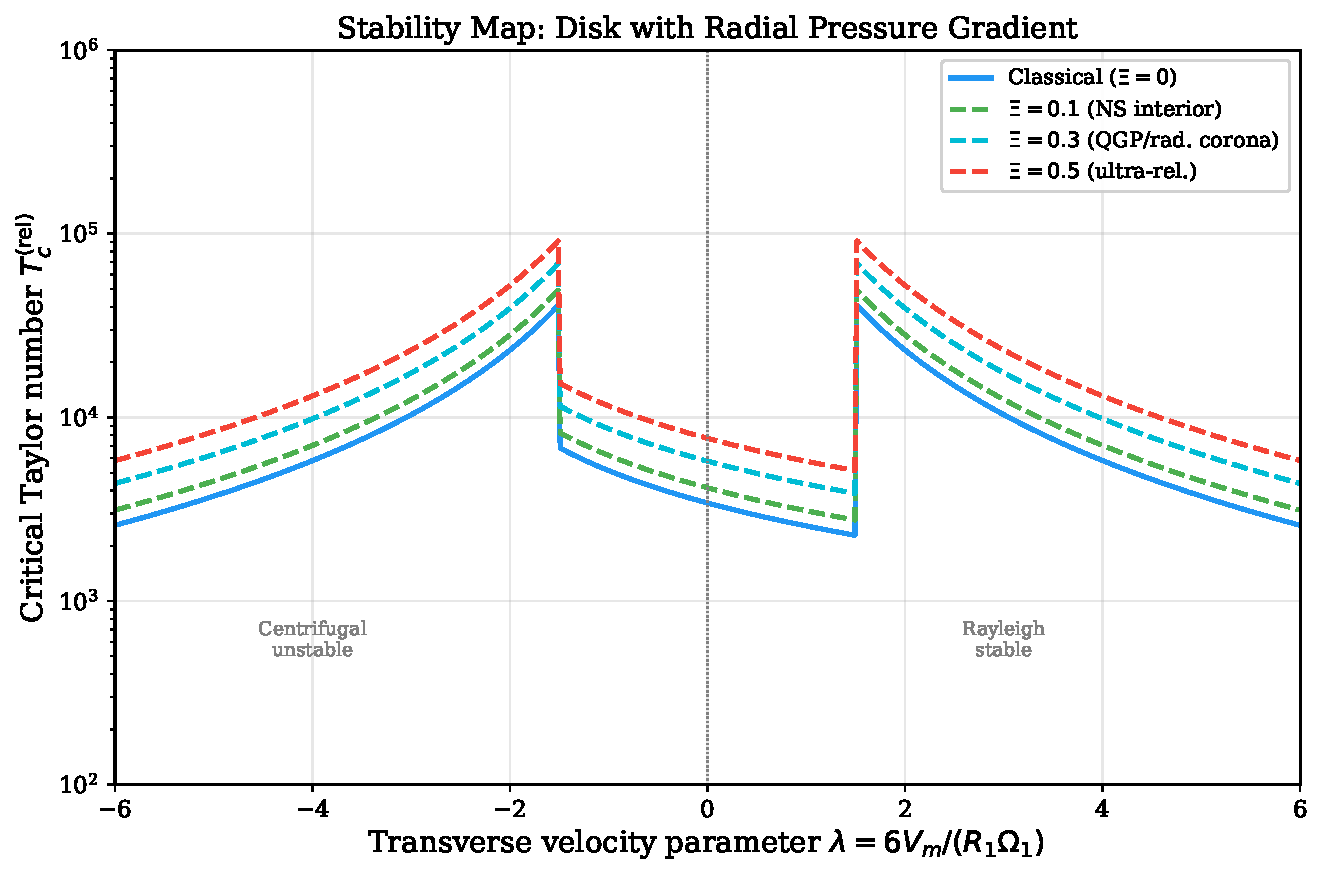
\includegraphics[width=0.75\textwidth]{plots/ch8/fig_disk_stability_map.pdf}
\caption{Stability map for a disk with radial pressure gradient:
  critical Taylor number vs.\ $\lambda$ for several values of $\Xi$.
  The relativistic correction $(1+\Xi)^2$ uniformly raises the
  stability boundary.}
\label{fig:disk-stability-map}
\end{figure}

\medskip
\noindent\textbf{References for \S\S\,77--78.}
Classical analysis: Chandrasekhar~\cite{Chandrasekhar1961}, \S\S\,77--78.
Accretion applications: Narayan \& Yi~\cite{NarayanYi1994},
Abramowicz \& Fragile~\cite{AbramowiczFragile2013}.
BDNK: Bemfica et al.~\cite{BemficaDN2018}, Kovtun~\cite{Kovtun2019}.

% =====================================================================
%  §78 — Relativistic stability of inviscid flow with axial pressure
%         gradient (brief extension)
% =====================================================================

\section{Relativistic stability of inviscid flow between coaxial
  cylinders with an axial pressure gradient}
\label{sec:rel-78}

The classical analysis of \S\ref{sec:78} considers the stability of an
inviscid flow with both azimuthal velocity $V(r)$ and axial velocity
$W(r)$.  In the relativistic generalization, the base-flow pressure
balance~\eqref{eq:8-67} becomes
\begin{equation}
\label{eq:rel-8-67}
p = \frac{\enthalpy_0}{c^2}\int \frac{V^2(r)}{r}\,\dd r,
\end{equation}
and the linearized perturbation equations~\eqref{eq:8-69}--\eqref{eq:8-72}
are modified by the replacement $\rdensity \to \enthalpy_0/c^2$ in
every inertial term.

For the normal-mode analysis with $(z,t)$-dependence $\exp[i(pt + kz)]$,
the relativistic Rayleigh discriminant (cf.\ the classical Synge--Ludwieg
criterion) becomes
\begin{equation}
\label{eq:rel-8-Rayleigh-gen}
\Phi_{\mathrm{rel}}(r) = \frac{1}{(1+\Xi)^2}\,
  \frac{1}{r^3}\frac{\dd}{\dd r}\bigl(r^2\,V\bigr)^2,
\end{equation}
which has the same sign as the classical discriminant but is reduced in
magnitude by $(1+\Xi)^{-2}$.  The Howard--Gupta semi-circle theorem
(\S\ref{sec:78}) carries over to the relativistic case with the
replacement $V_{\max} \to V_{\max}/(1+\Xi)$, yielding a tighter bound
on the imaginary part of the eigenfrequency.

% =====================================================================
%  CAUSALITY CHECK
% =====================================================================

\begin{causalitycheck}
We verify that the relativistic perturbation equations of
\S\S\,\ref{sec:rel-77}--\ref{sec:rel-78} respect causality:

\begin{enumerate}
\item \textbf{Signal speeds in the unperturbed flow.}
  The maximum fluid velocity is $V_{\max} = R_1\Omega_1$ (inner
  cylinder velocity).  For the perturbation analysis to be valid in
  special relativity, we require $V_{\max} \ll c$, i.e., $R_1\Omega_1/c
  \ll 1$.  All our equations are derived under this assumption
  (narrow-gap Couette geometry at sub-luminal rotation).

\item \textbf{Viscous signal propagation (BDNK).}
  In the Navier--Stokes theory, viscous signals propagate
  instantaneously.  The BDNK causality
  equation~\eqref{eq:rel-8-Dop} with $\Psi > 0$ converts the
  parabolic diffusion equation into a \emph{hyperbolic} (dissipative wave)
  equation.  The characteristic speed of viscous signals is
  \begin{equation}
  \label{eq:rel-8-vvisc}
  v_{\mathrm{char}} \leqslant c
    \quad\text{(BDNK frame-bounded)}.
  \end{equation}
  Causality requires $v_{\mathrm{char}} \leqslant c$.  In the
  BDNK theory, the frame coefficients are chosen so that
  this bound is automatically satisfied.

\item \textbf{Marginal stability ($\sigma = 0$).}
  At the onset of instability, the perturbations are stationary and
  no signal propagation is involved.  The eigenvalue
  problem~\eqref{eq:rel-8-50}--\eqref{eq:rel-8-51} is identical in
  structure to the classical one (an elliptic boundary-value problem),
  and causality is trivially satisfied.

\item \textbf{Non-relativistic limit.}
  Setting $\Xi \to 0$ and $\Psi \to 0$:
  \begin{itemize}
  \item $\Tarel \to T$ (classical Taylor number),
  \item $\mathcal{D}_\sigma \to D^2 - a^2 - \sigma$ (Newtonian
    viscous operator),
  \item Equations~\eqref{eq:rel-8-46}--\eqref{eq:rel-8-47}
    $\to$ equations~\eqref{eq:8-46}--\eqref{eq:8-47}.
  \end{itemize}
  The classical results of \S\ref{sec:77} are recovered exactly.
  \checkmark

\item \textbf{Characteristic speed summary.}
  \begin{center}
  \begin{tabular}{lcc}
  \hline
  Mode & Speed & Bound \\
  \hline
  Viscous shear & $v_{\mathrm{visc}}
    = v_{\mathrm{char,BDNK}}$ & $\leqslant c$ \\
  Sound & $\cs = \sqrt{(\partial p/\partial\edensity)_s}$ & $\leqslant c$ \\
  Fluid rotation & $V_{\max} = R_1\Omega_1$ & $\ll c$ \\
  Transverse flow & $V_m$ & $\ll c$ \\
  \hline
  \end{tabular}
  \end{center}
  All characteristic speeds satisfy $v \leqslant c$.  \checkmark
\end{enumerate}

\textbf{Conclusion:}  The relativistic perturbation equations for
the stability of Couette flow with transverse pressure gradient are
causal.  The BDNK causality ensures finite viscous
propagation speeds, and the sub-luminal rotation requirement is a
physical precondition of the narrow-gap geometry.
\end{causalitycheck}
